%------------------- Shafts -------------------%
\subsection{Shaft Analysis} 
\label{subsec:shaft}

%------------------------------ Inputs and Outputs ------------------------------%
\subsubsection{Inputs and Outputs}
There are three shafts in each robot leg: the hip control shaft and the knee control shaft, which are both inside the chassis and attached to a motor, and the exterior knee shaft, found outside the chassis. The shafts do not rotate continuously at high speeds; instead they oscillate and move at slow speeds. For this reason, a simple static force analysis was performed. The inputs include all the forces and torques applied to each shaft and the lengths of the portions of the shaft. The desired output is the diameter.

%------------------------------ CONSTANTS and Parameters ------------------------------%
\subsubsection{Constants and Parameters}

A minimum safety factor of 2.5 was chosen, as the selected material is well known but some of the applied forces, namely the force applied from the leg member onto the shaft, could vary due to the terrain \cite{juvinall_fundamentals_2012}. For example, vandalism, obstacles or shortcomings with the control system could cause slight impact forces to be felt at the shaft. 

Stress concentration factors were selected for the steps and keyways on the shafts. They were chosen as per the figures provided in Juvinall \cite{juvinall_fundamentals_2012}. For keyways, only fatigue stress concentration factors were provided, thus the static values were deduced from those values using the relations provided in the textbook.

There are many parameters affecting the shaft analysis such as its length. For the analysis, the total length was divided in multiple parts, such as the bearing thickness, pulley or hip plate thickness, torsion spring width and flange collar width. The other parameters are the various forces and torques applied to the shafts, which have been found in the modelling and in the analysis of the belt and pulleys in section \ref{subsec:belt}.


%------------------------------ Assumptions ------------------------------%
\subsubsection{Assumptions and Simplifications}

The analysis of the shafts is done at the worst case scenario, where the legs are fully extended (meaning higher torques and moments). It is also assumed that we are looking at the moment were the leg is lifting itself off the ground, meaning that the shafts experience forces from the ground and also the maximum applied torque from the motor as it is fighting the spring torque.

It was assumed that forces are applied at the middle of shaft components (for example, forces at bearings or pulleys). 
Another simplification that was made was to apply the axial force (created by friction forces at the foot) everywhere in the shaft, as it could be applied in either direction and load any part of the shaft.
It was also assumed that the force applied by the leg onto the shafts is vertical to the ground, as the largest component of the normal force is likely to be in that direction.
Finally, as there are many larger forces acting on the shafts, and these are computed for worse case scenarios, the weight of the shaft assembly itself was neglected when calculating bearing forces.


%------------------------------ Materials ------------------------------%
\subsubsection{Material Selection}
The selected material for all three shafts is marine grade stainless steel 316, as it is a common material used in marine applications and is often used for pump shafts. The minimum yield strength of this material is of about 205 MPa, thus we shall use a value of 240 MPa for a shaft with a cold finish \cite{metal_supermarkets_marine_2017}.


%------------------------------ Stress Analysis and FBDS ------------------------------%
\subsubsection{Stress Analysis and Free-Body Diagrams}
The following sections show the equations used for the static stress analysis of each shaft. A sample calculation is also provided after. It was decided not to perform a deflection and slope analysis as the shafts will be quite short and will not deflect much. A fatigue analysis was considered, however the robot will be moving quite slowly and will not have long operating hours. Thus, the complexity of this analysis was deemed unnecessary for this application.

%------------------------------ Knee ------------------------------%
\sssubsection{Exterior Knee Shaft}

Before presenting the free-body diagram for this shaft, some of the applied forces must be looked at more closely. As a worst case scenario, the calculations were made for when the robot was on a slope, thus creating additional moments on the shaft due to the added friction force. Figure \ref{fig:shaft_knee_friction} shows a simplified diagram of the tibia, and how moments in two planes are created at the knee shaft.

\begin{figure}
    \centering
    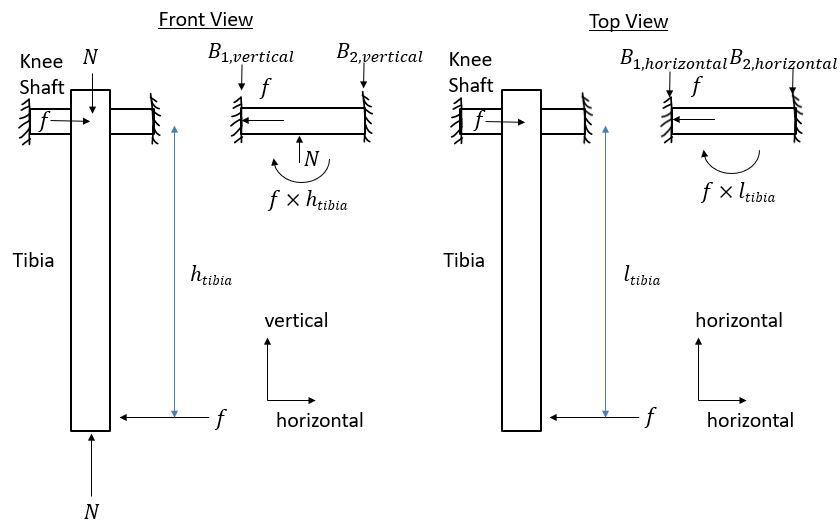
\includegraphics[width=0.9\textwidth]{4_Analysis/img/Shafts/ShaftKneeFriction.JPG}
    \caption{Exterior knee shaft - Friction moments}
    \label{fig:shaft_knee_friction}
\end{figure}

where $f$ is the friction force at the foot, $l_{tibia}$ is the horizontal extended length of the tibia (parallel to the ground) and $h_{tibia}$ is the vertical height of the tibia (perpendicular to the ground).

A side view of the pulley is shown in Figure
\ref{fig:shaft_knee_side}. It shows the various angles related to the leg position and the belt. The coordinate system is chosen to have the x direction in line with the thigh. As the pulleys were chosen to be the same size (no reduction), the angles of the belt $\delta_1$ and $\delta_2$ are both zero. The angle $\theta$ is equal to the thigh angle plus 90 degrees. 

\begin{figure}
    \centering
    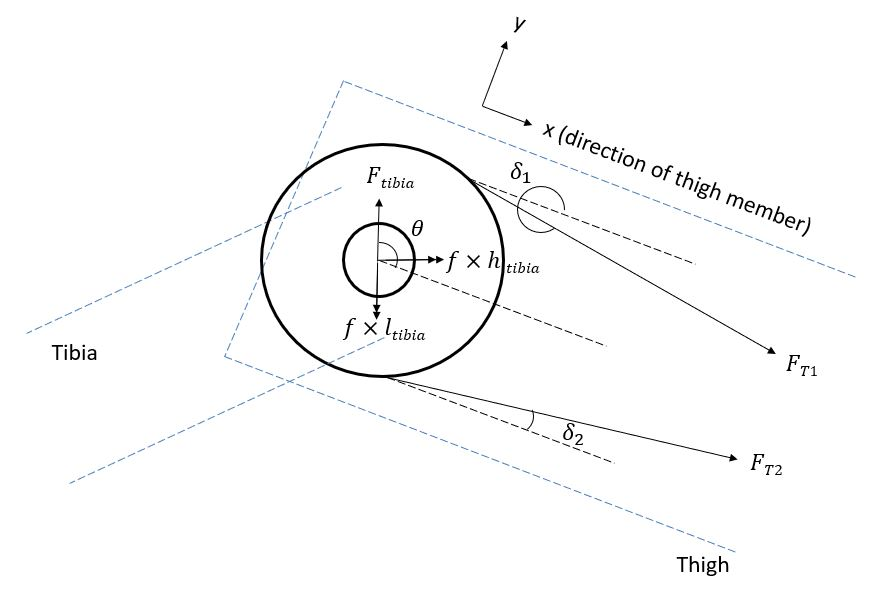
\includegraphics[width=0.9\textwidth]{4_Analysis/img/Shafts/ShaftKneeSide.JPG}
    \caption{Exterior knee shaft - Side section view of pulley (bearing reaction forces not visible in view}
    \label{fig:shaft_knee_side}
\end{figure}

$F_{T1}$ and $F_{T2}$ are the belt tension forces. The value $F_{tibia}$ (force of leg on shaft) is found using a force balance on the tibia, as shown in Figure \ref{fig:shaft_knee_tibia} and Equation \ref{eq:shaft_knee_Ftibia}, where $N$ is the normal force on the foot and $m_{foot}$ is the weight of the tibia lumped at the foot (as a worst case scenario for leg movement).

\begin{figure}
    \centering
    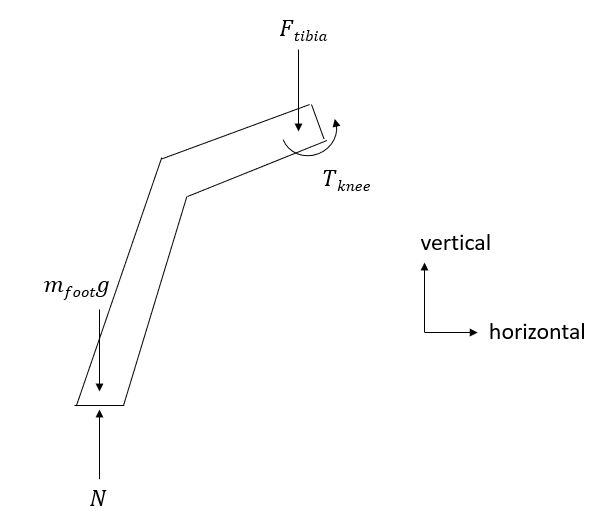
\includegraphics[width=0.6\textwidth]{4_Analysis/img/Shafts/ShaftKneeTibia.JPG}
    \caption{Exterior knee shaft - Tibia free-body diagram}
    \label{fig:shaft_knee_tibia}
\end{figure}

\begin{equation}
    \sum F_{vertical}=0:\;\;\;F_{tibia}=N-m_{foot} g
    \label{eq:shaft_knee_Ftibia}
\end{equation}

Finally, the exterior knee shaft succumbs to the forces shown in the free-body diagrams in Figures \ref{fig:shaft_knee_fbd1} and \ref{fig:shaft_knee_fbd2}.

\begin{figure}
    \centering
    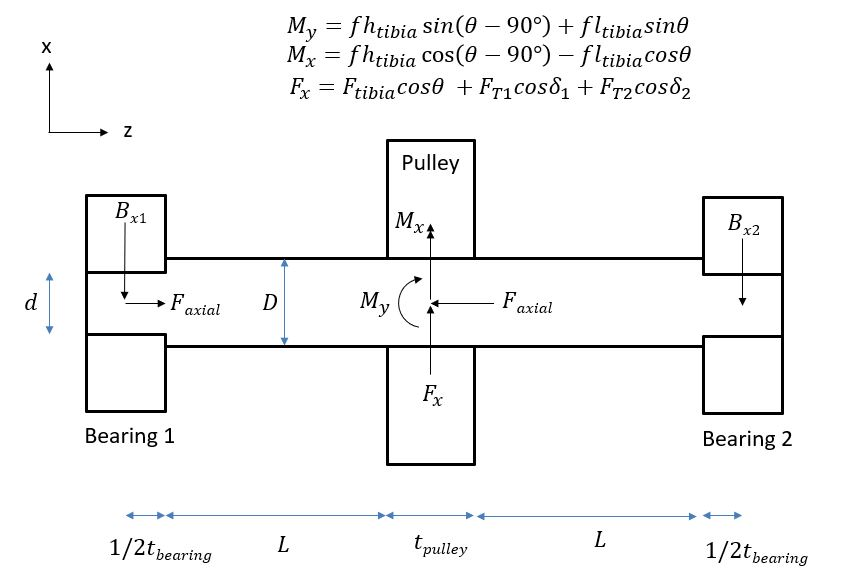
\includegraphics[width=0.9\textwidth]{4_Analysis/img/Shafts/ShaftKneeXZ.JPG}
    \caption{Exterior knee shaft - Free-body diagram in X-Z plane}
    \label{fig:shaft_knee_fbd1}
\end{figure}

\begin{figure}
    \centering
    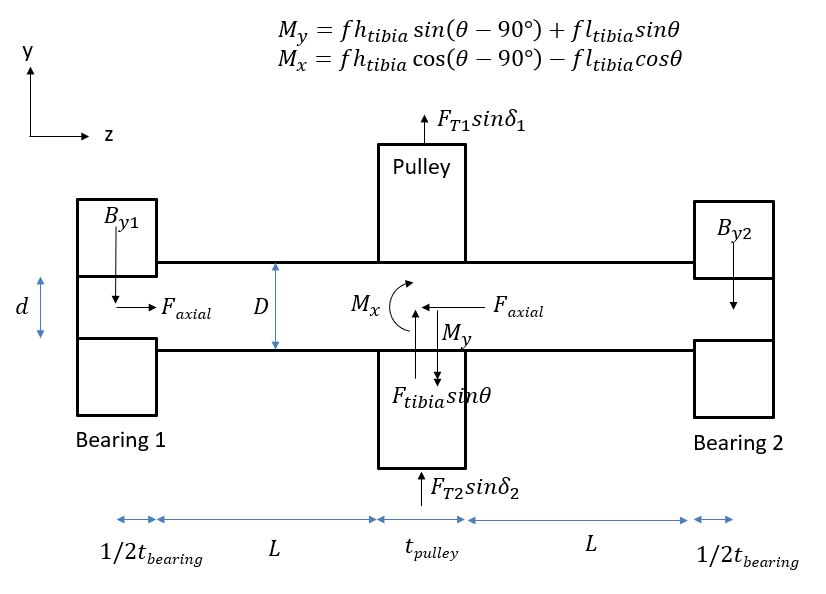
\includegraphics[width=0.8\textwidth]{4_Analysis/img/Shafts/ShaftKneeYZ.JPG}
    \caption{Exterior knee shaft - Free-body diagram in Y-Z plane}
    \label{fig:shaft_knee_fbd2}
\end{figure}

where $B_{yi}$ and $B_{xi}$ are the forces at the bearings, $F_{axial}$ is the axial force in the shaft which is equal to the friction force at the foot $f$, $t_{bearing}$ is the width of the bearing, $L$ is a length determined by the width of the thigh and thus the spacing of the knee plates, $t_{pulley}$ is the thickness of the pulley and $d$ and $D$ are the diameters of the shaft.

To start the analysis, the resulting forces applied at the bearings were calculated using sum of forces and moments.

\begin{gather}
\begin{split}
    \sum M_{x_{@Bearing 1}}=0:  B_{y2}=
    \\
    \frac{(1/2t_{bearing}+L+1/2t_{pulley})(F_{tibia}\sin{\theta}+F_{t1}\sin{\delta_1}+F_{t2}\sin{\delta_2})-fh_{tibia}\cos{(\theta-90^{\circ})}+fl_{tibia}\cos{\theta}}{t_{bearing}+2L+t_{pulley}}
\end{split}
    \\
    \begin{split}
          \sum M_{y_{@Bearing 1}}0:  B_{x2}=
          \\
          \frac{(1/2t_{bearing}+L+1/2t_{pulley})(F_{tibia}\cos{\theta}+F_{t1}\cos{\delta_1}+F_{t2}\cos{\delta_2})-fh_{tibia}\sin{(\theta-90^{\circ})}-fl_{tibia}\sin{\theta}}{t_{bearing}+2L+t_{pulley}}  
    \end{split}
    \\
    \sum F_x=0: B_{x1}=F_{tibia}\cos{\theta}+F_{t1}\cos{\delta_1}+F_{t2}\cos{\delta_2}-B_{x2}
    \\
    \sum F_y=0: B_{y1}=F_{tibia}\sin{\theta}+F_{t1}\sin{\delta_1}+F_{t2}\sin{\delta_2}-B_{y2}
\end{gather}

These values were used to create shear force and bending moment diagrams over the length of the shaft. These are shown in Figure \ref{fig:shaft_knee_diagrams}.

\begin{figure}
    \centering
    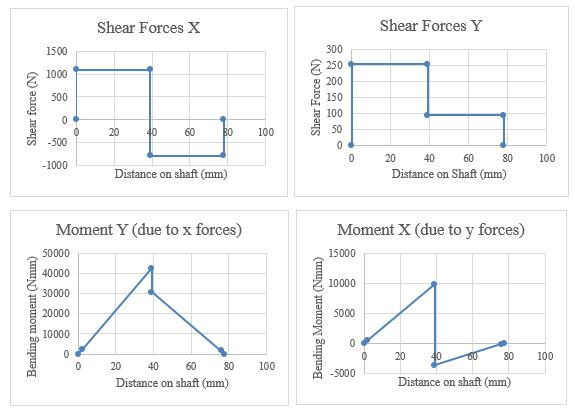
\includegraphics[width=0.8\textwidth]{4_Analysis/img/Shafts/ShaftKneeDiagrams.JPG}
    \caption{Exterior knee shaft - Shear force and bending moment diagrams}
    \label{fig:shaft_knee_diagrams}
\end{figure}

Critical points on the shaft were then selected and analyzed for strength. These critical points are the steps in the shaft and the maximum bending moment point located at the pulley. The forces and moments acting in perpendicular directions were added together using the following formula to find a resultant.

\begin{equation}
    F_{total}=\sqrt{F_x^2+F_y^2}
    \;\;\;\;
    M_{total}=\sqrt{M_x^2+M_y^2} \label{eq:Ftotal}
\end{equation}{}

The bending stress, transverse shear stress and axial stress were then found using the following formulas \cite{juvinall_fundamentals_2012}. In this case, no torsion is applied on the shaft since the pulley is not fixed to the shaft. It is the reason why transverse shear stresses are taken into account.

\begin{gather}
    \tau_{transverse\;shear}=\frac{4}{3} (\frac{k_t F_{total}}{\frac{\pi{}d^2}{4}})
    \\
    \sigma_{bending}=\frac{32k_tM_{total}}{\pi{}d^3} \label{eq:shaft_bending_stress}
    \\
    \sigma_{axial}=\frac{k_tF_{axial}}{\frac{\pi{}d^2}{4}} \label{eq:shaft_axial_stress}
\end{gather}

where $k_t$ are the stress concentration factors for the stress mode being evaluated, at the observed point on the shaft. These values were obtained from the Juvinall textbook \cite{juvinall_fundamentals_2012}. The value for transverse shear was estimated by taking the value for torsion shear. 

The equivalent stress was then calculated using the Von Mises formula \cite{juvinall_fundamentals_2012}, and this was compared to the yield strength of the chosen material to ensure the safety factor is met:

\begin{gather}
    \sigma_{equivalent}=\sqrt{(\sigma_{bending}+\sigma_{axial})^2+3\tau_{transverse\;shear}^2}
    \\
    SF=\frac{S_y}{\sigma_{equivalent}}
\end{gather}

where $\sigma_{equivalent}$ is the equivalent Von Mises stress, $S_y$ is the yield stress of the material and SF is the safety factor.

%------------------------------ Hip ------------------------------%
\sssubsection{Hip Control Shaft}
The friction force created by walking on a slope would cause additional moments to be created on this shaft as well. Figure \ref{fig:shaft_hip_friction} shows a simplified diagram of the full leg, and how moments in two planes are created at the hip control shaft.

\begin{figure}
    \centering
    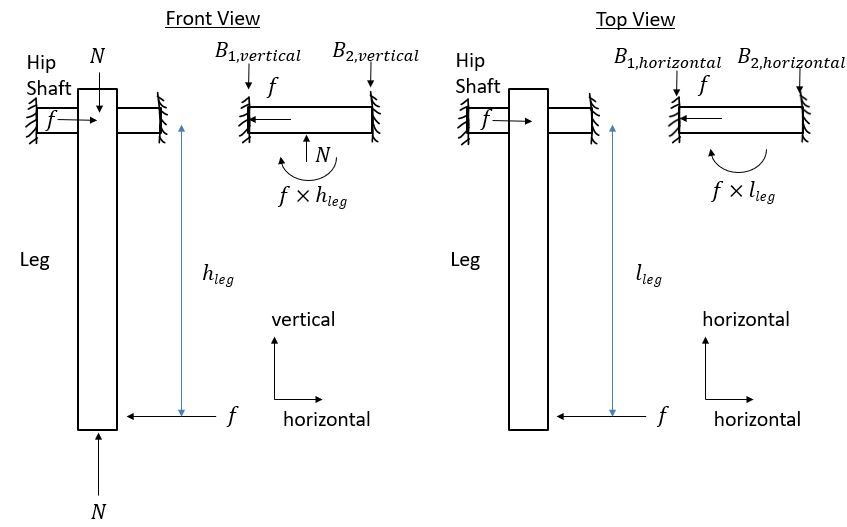
\includegraphics[width=0.9\textwidth]{4_Analysis/img/Shafts/ShaftHipFriction.JPG}
    \caption{Hip control shaft - Friction moments}
    \label{fig:shaft_hip_friction}
\end{figure}

where $f$ is the friction force at the foot, $l_{leg}$ is the horizontal extended length of the leg (parallel to the ground) and $h_{leg}$ is the vertical height of the leg (perpendicular to the ground).

The value of the leg force acting on the hip shaft, $F_{thigh}$, is found using a force balance on the thigh, as shown in Figure \ref{fig:shaft_hip_thigh} and Equation \ref{eq:shaft_hip_Fthigh}, where $m_{knee}$ is the weight of the thigh lumped at the knee (as a worst case scenario for leg movement).

\begin{figure}
    \centering
    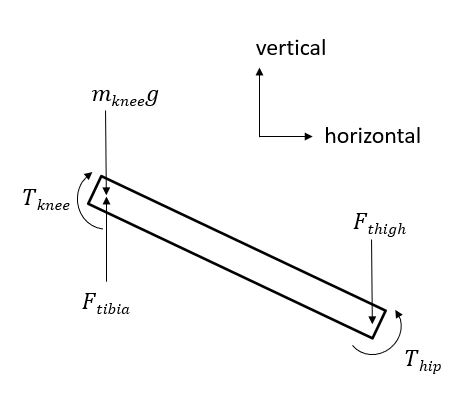
\includegraphics[width=0.7\textwidth]{4_Analysis/img/Shafts/ShaftHipThigh.JPG}
    \caption{Hip control shaft - Thigh free-body diagram}
    \label{fig:shaft_hip_thigh}
\end{figure}

\begin{equation}
    \sum F_{vertical}=0:\;\;\;F_{thigh}=F_{tibia}-m_{knee} g
    \label{eq:shaft_hip_Fthigh}
\end{equation}

Thus, the hip control shaft succumbs to the forces shown in the free-body diagrams in Figures \ref{fig:shaft_hip_fbd1} and \ref{fig:shaft_hip_fbd2}. The coordinates were chosen as x being parallel to the ground and y being vertical to the ground.

\begin{figure}
    \centering
    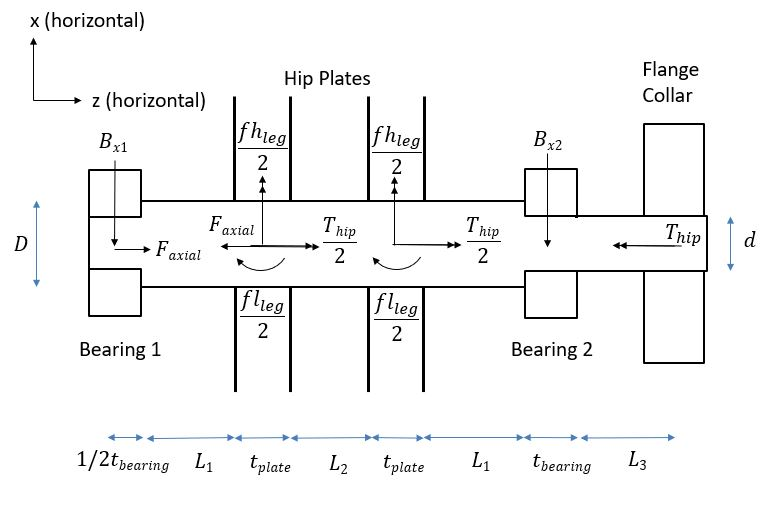
\includegraphics[width=0.9\textwidth]{4_Analysis/img/Shafts/ShaftHipXZ.JPG}
    \caption{Hip control shaft - Free-body diagram in X-Z plane}
    \label{fig:shaft_hip_fbd1}
\end{figure}

\begin{figure}
    \centering
    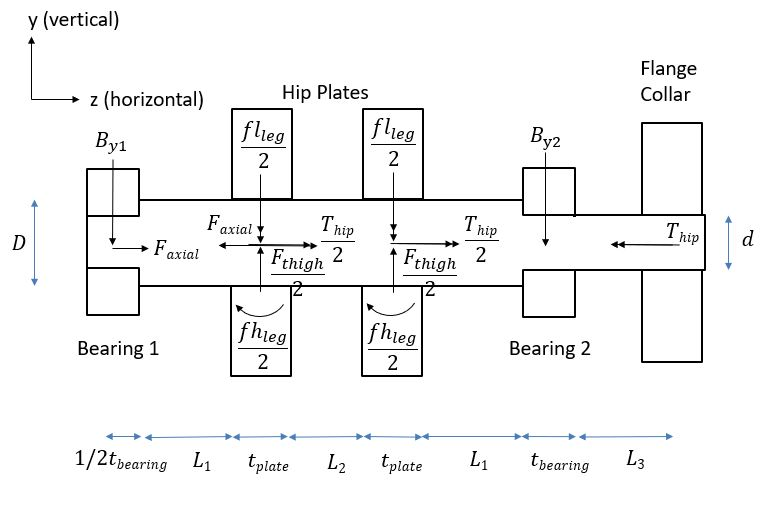
\includegraphics[width=0.9\textwidth]{4_Analysis/img/Shafts/ShaftHipYZ.JPG}
    \caption{Hip control shaft - Free-body diagram in Y-Z plane}
    \label{fig:shaft_hip_fbd2}
\end{figure}

where the variables remain similar to the exterior knee shaft, however $t_{hip}$ is the torque provided by the motor at the hip, $L_1$ is the width of the torsion spring which is positioned at that location on the shaft, $L_2$ is a length determined by the spacing of the hip plates, $L_3$ is the distance between bearing 2 and the middle of the flange collar attached to the harmonic drive and $t_{plate}$ is the width of the hip plates.

Similarly to the exterior knee shaft, sum of forces and moments is used to find equations for the forces at the bearings. 

\begin{gather}
    \sum M_{x_{@Bearing 1}}=0:  B_{y2}=\frac{\frac{F_{thigh}}{2}(t_{bearing}+2L_1+2t_{plate}+L_2)-fh_{leg}}{t_{bearing}+2L_1+2t_{plate}+L_2} \label{eq:hip_bearing1}
    \\
    \sum M_{y_{@Bearing 1}}=0:  B_{x2}=-\frac{fl_{leg}}{t_{bearing}+2L_1+2t_{plate}+L_2}
    \\
    \sum F_x=0: B_{x1}=-B_{x2}
    \\
    \sum F_y=0: B_{y1}=F_{thigh}-B_{y2} \label{eq:hip_bearing2}
\end{gather}

The shear force and bending moment diagram were then created and are shown in Figure \ref{fig:shaft_hip_diagrams}. This shaft also encounters torsion as the hip plates are fixed on the shaft by keys. The torsion diagram is also shown in Figure \ref{fig:shaft_hip_diagrams}. As there are two hip plates taking the torque applied by the motor, it was assumed that each took about half the torque. This should not affect the calculation of stress at the critical point, as the full torque is still used for the stress at the first plate, and will determine the diameter.

\begin{figure}
    \centering
    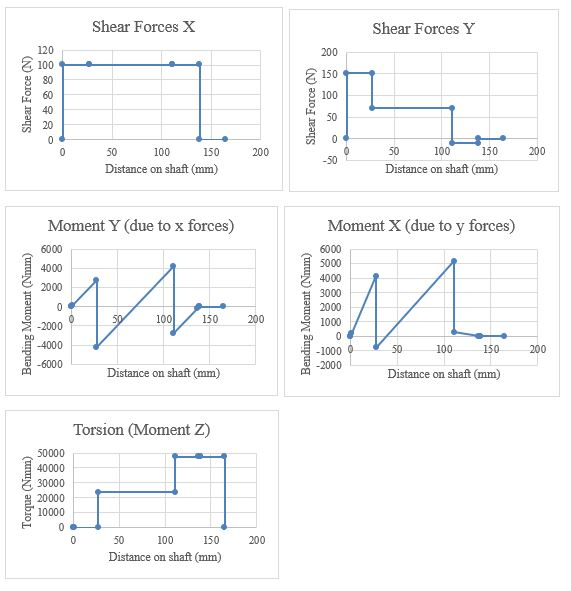
\includegraphics[width=0.7\textwidth]{4_Analysis/img/Shafts/ShaftHipDiagrams.JPG}
    \caption{Hip control shaft - Shear force, bending moment and torque diagrams}
    \label{fig:shaft_hip_diagrams}
\end{figure}

The critical points on the shaft are the two steps, as well as the keyways at both hip plates and the flanged collar (for the harmonic drive). The strength analysis was done using the same equations as for the exterior knee shaft, with the exception of the following additional torsion stress equation \cite{juvinall_fundamentals_2012}.

\begin{gather}
    \tau_{torsion}=\frac{16k_tT}{\pi{}d^3} \label{eq:shaft_torsion_stress}
\end{gather}

where $k_t$ is the stress concentration factor specific to torsion.

In this situation, the torsional shear stress is much larger than the transverse shear stress and thus the transverse shear stress was neglected. This decision is founded in the fact that the maximum torsion shear stress is at the shaft surface whereas the maximum transverse shear stress is in the middle of the shaft. They are not applied at the same point and are thus not to be considered as a summation. The Von Mises equation becomes:

\begin{gather}
    \sigma_{equivalent}=\sqrt{(\sigma_{bending}+\sigma_{axial})^2+3\tau_{torsion}^2} \label{eq:shaft_vonmises}
\end{gather}


%------------------------------ Hip-Knee ------------------------------%
\sssubsection{Knee Control Shaft}
This shaft does not take any force or moment from the leg. Thus, the knee control shaft succumbs to the forces shown in the free-body diagrams in Figures \ref{fig:shaft_hipknee_fbd1} and \ref{fig:shaft_hipknee_fbd2}. The coordinates are the same as for the exterior knee shaft, with x in the direction of the thigh member. In this case, the angle of the belt tension forces is the same as for the exterior knee shaft, with an added 180 degrees (as they are in the opposite direction). Those forces are shown in the positive x or y direction, as they depend on the angles.

\begin{figure}
    \centering
    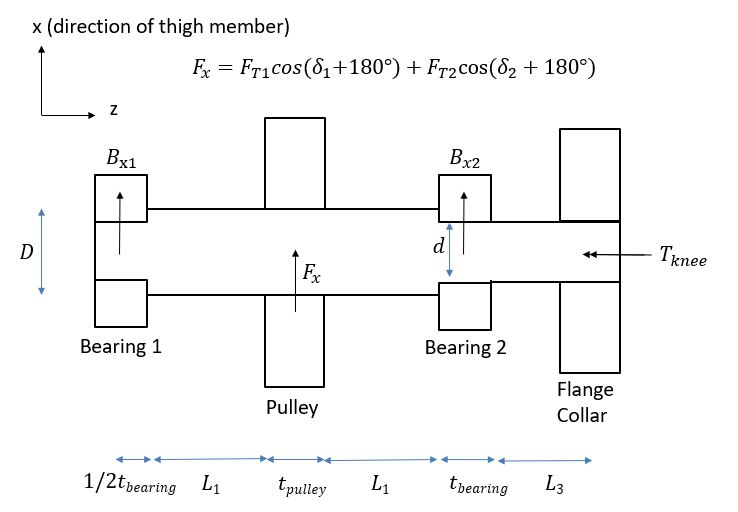
\includegraphics[width=0.8\textwidth]{4_Analysis/img/Shafts/ShaftHipKneeXZ.JPG}
    \caption{Knee control shaft - Free-body diagram in X-Z plane}
    \label{fig:shaft_hipknee_fbd1}
\end{figure}

\begin{figure}
    \centering
    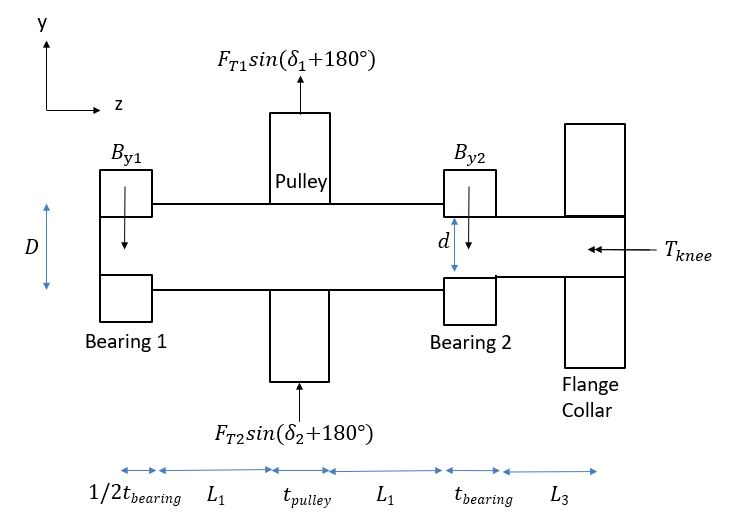
\includegraphics[width=0.8\textwidth]{4_Analysis/img/Shafts/ShaftHipKneeYZ.JPG}
    \caption{Knee control shaft - Free-body diagram in Y-Z plane}
    \label{fig:shaft_hipknee_fbd2}
\end{figure}

where variables are similar to the other shafts, with $T_{knee}$ the torque provided by the motor, $L_1$ is the width of the torsion spring and $L_3$ is the distance from the bearing 2 to the middle of the flange collar.

Similarly to the other shafts, sum of forces and moments is used to find equations for the forces at the bearings. 

\begin{gather}
    \sum M_{x_{@Bearing 1}}=0:  B_{y2}=\frac{(1/2 t_{bearing}+L_1+1/2 t_{pulley} )(F_{T1} \sin{(\delta_1+180)}+F_{T2} \sin{(\delta_2+180)})}{(t_{bearing}+2L_1+t_{pulley} )} \label{eq:shaft_kneehip_1}
    \\
    \sum M_{y_{@Bearing 1}}=0:  B_{x2}=-\frac{(1/2 t_{bearing}+L_1+1/2 t_{pulley} )(F_{T1} \cos{(\delta_1+180)}+F_{T2} \cos{(\delta_2+180)})}{(t_{bearing}+2L_1+t_{pulley} )}
    \\
    \sum F_x=0: B_{x1}=-F_{T1}\cos(\delta_1+180)-F_{T2} \cos(\delta_2+180)-B_{x2}
    \\
    \sum F_y=0: B_{y1}=F_{T1}\sin(\delta_1+180)+F_{T2} \sin(\delta_2+180)-B_{y2}
\end{gather}

The shear force, bending moment and torque diagrams were then created and are shown in Figure \ref{fig:shaft_hipknee_diagrams}. 

\begin{figure}
    \centering
    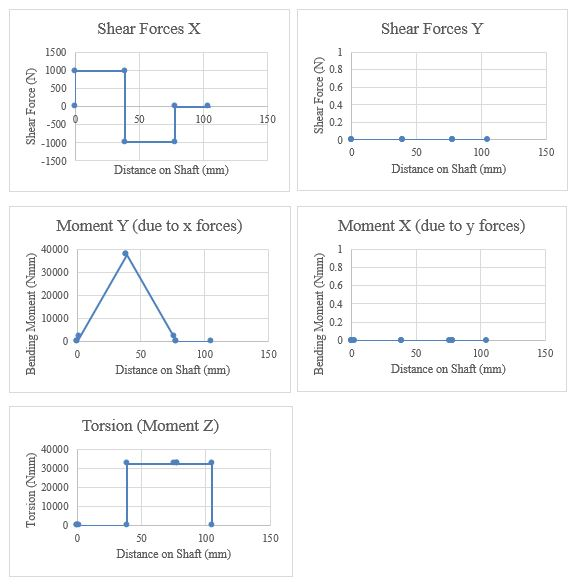
\includegraphics[width=0.8\textwidth]{4_Analysis/img/Shafts/ShaftHipKneeDiagrams.JPG}
    \caption{Knee control shaft - Shear force, bending moment and torque diagrams}
    \label{fig:shaft_hipknee_diagrams}
\end{figure}

The critical points on the shaft are the two steps, as well as the keyway at the pulley and the flanged collar (for the harmonic drive). The strength analysis was done using the previous equations. Once again, as torsion is applied to the shaft, the transverse shear is not used in the analysis.

%------------------------------ Example ------------------------------%
\sssubsection{Example Calculation} \label{sec:shaft_example}

The following is a calculation to find the required shaft diameter of the hip control shaft based on the applied forces and length of the shaft. This shaft is the most critical as it succumbs to the largest torque.

First, we must find the forces acting on the bearings using Equations \ref{eq:hip_bearing1} to \ref{eq:hip_bearing2}. We first find the value of $F_{thigh}=161.6 N$ using a combination of Equation \ref{eq:shaft_knee_Ftibia} and \ref{eq:shaft_hip_Fthigh} with the values $m_{foot}=0.25 kg$, $m_{knee}=0.50 kg$ and $N=169 N$ (maximum expected normal force, as calculated in the slope analysis Section \ref{sec:modelling_slope}). The friction force at the foot from the slope analysis is $f=51.7 N$ and from the leg lengths and angles we get $h_{leg}=190.0 mm$ and $l_{leg}=268.6 mm$. The other values are a bearing thickness (length) $t_{bearing}= 3 mm$, a hip plate thickness of $t_{plate}=10 mm$, $L_1 = 20.8 mm$ is the width of the torsion springs at the hip, $L_2 = 75.5 mm$ is determined by the required length of the knee control shaft and $L_3=25 mm$ to give space for the flange collar. Now we get the forces on the bearings:

\begin{gather}
\begin{split}
    \sum M_{x_{@Bearing 1}}=0:  B_{y2}=
    \\
    \frac{\frac{161.6 N}{2}(3 mm+2(20.8 mm)+2(10 mm)+75.5 mm)-(51.7 N)(190.0 mm)}{3 mm+2(20.8 mm)+2(10 mm)+75.5 mm}=9.9 N 
\end{split}
    \\
    \sum M_{y_{@Bearing 1}}=0:  B_{x2}=-\frac{51.7 N(268.6 mm)}{3 mm+2(20.8 mm)+2(10 mm)+75.5 mm}=-100.3 N
    \\
    \sum F_x=0: B_{x1}=-B_{x2}=100.3 N
    \\
    \sum F_y=0: B_{y1}=161.6 N-(9.9 N)=151.8 N
\end{gather}

Note that some values are negative due to the moments created by the friction on the leg. The signs would be reversed if the friction was in the opposite direction.

The most critical point on the shaft is the step next to bearing 2, thus this is the point analysed here. From the creation of the force diagrams shown in Figure \ref{fig:shaft_hip_diagrams} we get that at its location of 136.9 mm from the middle of bearing 1, the bending moments are $M_x=14.8N$ and $M_y=-150.4N$. The torsion is equal to $T=47440 Nmm$ and the axial force is the friction force $F_{axial}=f=51.7N$. 
We use Equation \ref{eq:Ftotal} to get the total bending moment of $M=151.2 Nmm$.
Then Equations \ref{eq:shaft_torsion_stress}, \ref{eq:shaft_bending_stress} and \ref{eq:shaft_axial_stress} can be used to find the stresses at that point. Using the Juvinall textbook \cite{juvinall_fundamentals_2012}, the concentration factors are found to be 2.0 in bending, 2.1 in axial stress and 1.7 in torsion. A value of small diameter of $d=19.5 mm$ is assumed for now, and values of stress are verified later using the safety factor.

\begin{gather}
    \tau_{torsion}=\frac{16(1.7)(47440 Nmm)}{\pi{}(19.5 mm)^3}=55.4 MPa
    \\
    \sigma_{bending}=\frac{32(2.0)(151.2Nmm)}{\pi{}(19.5mm)^3}=0.42 MPa
    \\
    \sigma_{axial}=\frac{2.1(51.7N)}{\frac{\pi{}(19.5mm)^2}{4}}=0.36 MPa
\end{gather}

Then the Von Mises Equation \ref{eq:shaft_vonmises} is used to get the equivalent stress, and the safety factor is verified. The selected diameter gives the required safety factor and is therefore considered adequate.

\begin{gather}
    \sigma_{equivalent}=\sqrt{(0.42 MPa+0.36 MPa)^2+3(55.4 MPa)^2}=95.9 MPa
    \\
    SF=\frac{240 MPa}{95.9 MPa}=2.5
\end{gather}

Table \ref{tab:shaft} summarizes the bearing forces found for each shaft as well as the required diameters for each shaft. 

\begin{table}[H]
    \centering
    \caption{Calculated shaft diameters and forces at bearings}
    \label{tab:shaft}
    \begin{tabular}{c c c c}
        \\ \hline
        \textbf{Values} & \textbf{Exterior Knee Shaft} & \textbf{Hip Control Shaft} & \textbf{Knee Control Shaft}
        \\ \hline
        $B_{x1}$ [N] & 1095.4 & 100.3 & 967.2
        \\
        $B_{x2}$ [N] & 790 & -100.3 & 967.2
        \\
        $B_{y1}$ [N]& 252.6 & 151.8 & 0
        \\
        $B_{y2}$ [N]& -93.5 & 9.9 & 0
        \\
        $d$ [mm]& 13 & 19.5 & 17.5
        \\
        $D$ [mm]& 17 & 23.5 & 21.5
        \\ \hline
    \end{tabular}
\end{table}

%------------------------------ Critical Review ------------------------------%
\subsubsection{Critical Review}
The diameters found in Table \ref{tab:shaft} are realistic for the selected material and relatively small torques and bending moments. The exterior knee shaft has the smallest values as it does not succumb to torsion. As the hip control shaft succumbs to the largest torsion, it naturally has the biggest diameters. This shaft however has the smallest bearing forces as it does not have to resist to the belt tensions like the other two shafts.

%------------------------------ Parameterization ------------------------------%
\subsubsection{Parameterization}
The goal of the shaft parameterization will be to take inputs such as shaft lengths (based on other component sizes), torques and forces and find the required shaft diameters for those loads. An estimated diameter will be chosen and increased until a diameter that meets the safety factor is found. 